\section{Preverjanje predpostavk linearnega regresijskega modela}

Predpostavke linearnega regresijskega modela bomo preverili s pomočjo štirih \emph{diagnostičnih grafov}.
Če nekatere predpostavke nisi izpolnjene so lahko rezultati netočni.

\begin{figure}[h]
    \centering
    \begin{subfigure}[t]{0.49\textwidth}
        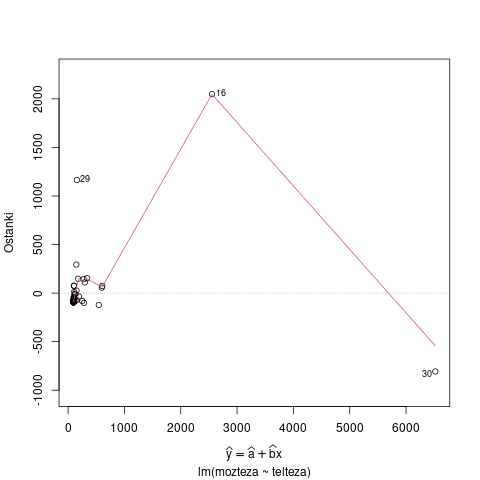
\includegraphics[width=\textwidth]{res/linearnost-modela.png}
        \caption{Linearnost modela}
        \label{img:linearnost-modela}
    \end{subfigure}
    \hfill
    \begin{subfigure}[t]{0.49\textwidth}
        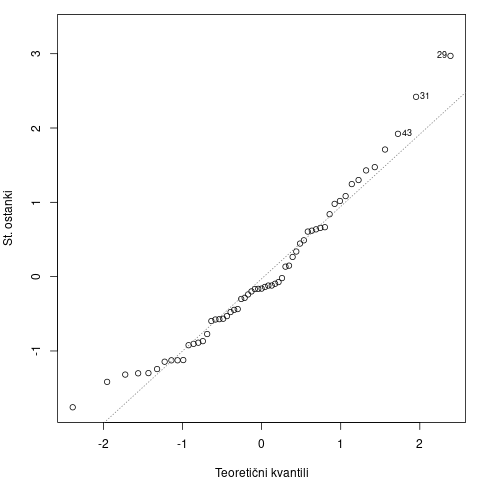
\includegraphics[width=\textwidth]{res/normalnost-porazdelitve.png}
        \caption{Normalnost porazdelitve}
        \label{img:normalnost-porazdelitve}
    \end{subfigure}

    \begin{subfigure}[t]{0.49\textwidth}
        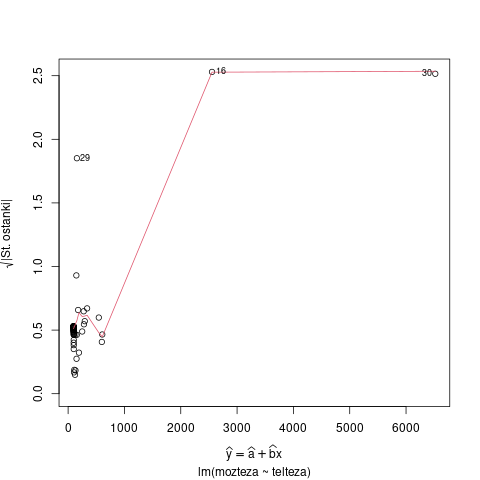
\includegraphics[width=\textwidth]{res/homogenost-variance.png}
        \caption{Homogenost variance}
        \label{img:homogenost-variance}
    \end{subfigure}
    \hfill
    \begin{subfigure}[t]{0.49\textwidth}
        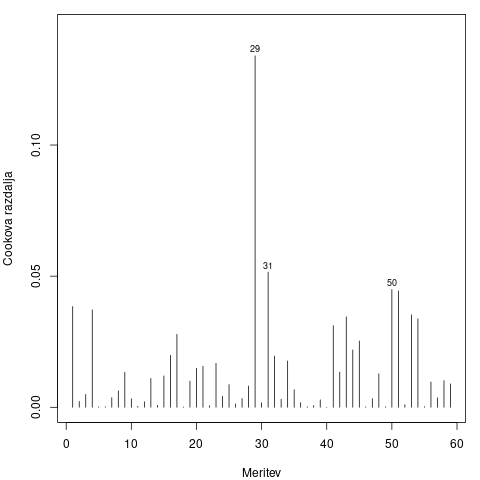
\includegraphics[width=\textwidth]{res/vpliv-tock-na-model.png}
        \caption{Vpliv točk na model}
        \label{img:vpliv-tock-na-model}
    \end{subfigure}
\end{figure}

Za izris grafov v funkciji \emph{plot()} izberemo model iz katerega želimo izrisati grafe
(v našem primeru \emph{model}), da ne želimo prikazati naslova (\emph{caption = ""}) in ann (\emph{ann = F}),
v funkciji \emph{title()} pa izberemo podatke za naslove x in y osi.

\newpage

\subsection{Graf za preverjanje linearnosti modela}

Graf \ref{img:linearnost-modela} smo narisali z ukazi:
\lstinputlisting[firstline=5,lastline=9,title=Generiranje grafa linearnosti modela
(glej kodo \ref{code:model})]{res/model.r}

\subsection{Graf normalnosti porazdelitve naključnih napak}

Graf \ref{img:normalnost-porazdelitve} smo narisali z ukazi:
\lstinputlisting[firstline=13,lastline=14,title=Generiranje grafa normalnosti porazdelitve
(glej kodo \ref{code:model})]{res/model.r}

\subsection{Graf homogenosti variance}

Graf \ref{img:homogenost-variance} smo narisali z ukazi:
\lstinputlisting[firstline=18,lastline=22,title=Generiranje grafa homogenosti variance
(glej kodo \ref{code:model})]{res/model.r}

\subsection{Graf vpliva posameznih točk na model}

Graf \ref{img:vpliv-tock-na-model} smo narisali z ukazi:
\lstinputlisting[firstline=26,lastline=27,title=Generiranje grafa vpliva točk na model
(glej kodo \ref{code:model})]{res/model.r}